\documentclass[10pt,a4paper]{article}
\usepackage[utf8]{inputenc}
\usepackage[T1]{fontenc}
\usepackage{lmodern}
\usepackage{geometry}
\geometry{margin=21mm,top=20mm,bottom=21mm}
\usepackage{amsmath,amssymb,graphicx,booktabs,tabularx,enumitem,microtype,xcolor,hyperref,float}
\hypersetup{colorlinks=true,linkcolor=blue!45!black,urlcolor=blue!45!black}
\usepackage{fancyhdr}
\pagestyle{fancy}\fancyhf{}\fancyhead[L]{A070 / v0.2.3 -- observational audit}\fancyhead[R]{DEVELOPMENT / NOT CERTIFIED}\fancyfoot[C]{\thepage}
\setlength{\headheight}{13.5pt}
\newcommand{\status}{\textbf{UNRESOLVED}}
\title{\vspace{-1.3em}A070 -- Axiale puls in een roterende watercilinder\\[2mm]
\large Frameanalyse, controledynamica en preregistratie voor v0.2.3}
\author{SST-Workbench onderzoeksnotitie}
\date{19 oktober 2026 -- \textbf{Observatie / plan, geen fysische certificatie}}
\begin{document}\maketitle\vspace{-2em}
\begin{abstract}
De opgenomen centrale structuur verandert zichtbaar na een rotorpuls, maar er is uit de enkele zijaanzichtvideo geen eenduidige axiale fase- of groepssnelheid terug te winnen. De video is een \emph{exploratory discovery sample}; een nieuwe proef moet de actuatietijd, materiaaladvectie, golfrespons en waterspiegel onafhankelijk meten. De fictieve of vooraf gekozen SST-lichtsnelheid en SST-kernparameters worden nergens gebruikt bij de analyse.
\end{abstract}
\section{Herkomst en kalibratie}
Video: \texttt{20260625\_020642\_1.mp4}, 3984 frames, 1080\,$\times$\,1920, afspeelsnelheid $29.9724\,\mathrm{fps}$; door de gebruiker opgegeven capture-rate $240\,\mathrm{fps}$. Een-op-een retentie van de originele frames wordt verondersteld. Controle met eventueel telefoonmetadata blijft open.
\begin{align}
S&=\frac{240}{29.9724}=8.00736, & t_{\mathrm{lab}}&=\frac{N_{\mathrm{frames}}}{240},\\
12\,\mathrm{s}\ \text{afspeeltijd}&\longrightarrow 1.499\,\mathrm{s}\ \text{opnametijd}, & T_{\rm rot}&\simeq\frac{14}{S}=1.748\,\mathrm s.
\end{align}
Het afgeleide achtergrondtoerental is $60/T_{\rm rot}\simeq34.3\,\mathrm{rpm}$; dit is consistent binnen de ruwe timingnauwkeurigheid met de genoemde motorlimiet van ongeveer $33\,\mathrm{rpm}$. De pulsaanvang \emph{ten opzichte van dit tijdstip} is onbekend. De laboratoriumtijd $t_{\rm lab}$ mag niet zonder fysieke toets worden gelijkgesteld met de veronderstelde universele SST-absolute tijd.

\begin{center}\begin{tabular}{lll}\toprule
Afmeting/parameter & Waarde & Bewijskwaliteit\\\midrule
Cilinderdiameter & $0.150\,\mathrm m$ & opgegeven\\
Cilinderhoogte & $0.300\,\mathrm m$ & opgegeven, \emph{niet} waterdiepte\\
Draaisnelheid & $\sim33$--$34\,\mathrm{rpm}$ & indirect uit ~14 s afspeeltijd\\
Waterdiepte $h$ & onbekend & moet gemeten worden\\
Rotorschijfdiameter/impulsduur & onbekend & ontbrekende randvoorwaarde\\
\bottomrule\end{tabular}\end{center}
\section{Geselecteerde waarneming}
\begin{figure}[H]\centering
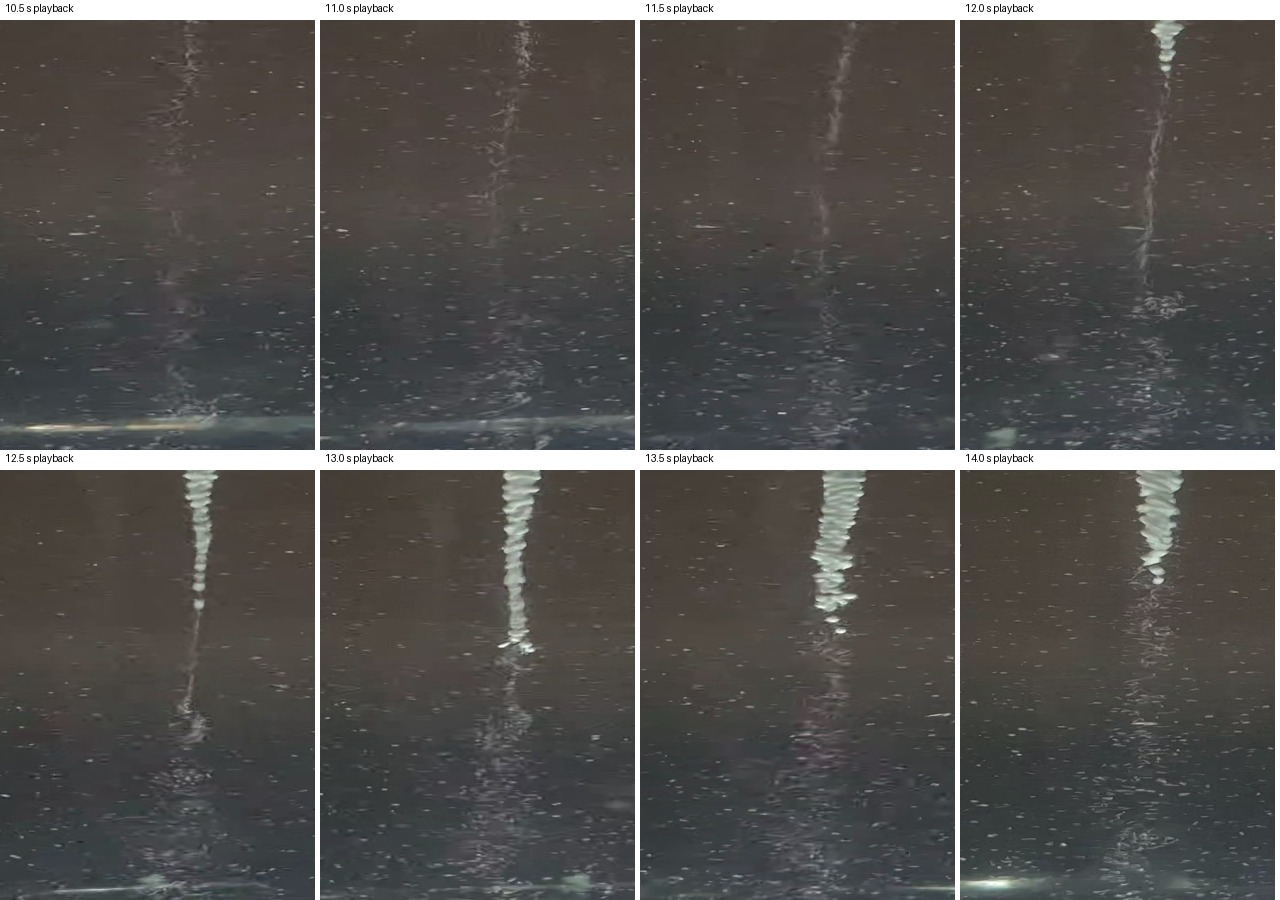
\includegraphics[width=.96\linewidth]{results/central_frames.jpg}
\caption{Dezelfde centrale beeldstrook, van 10.5 tot 14 s afspeeltijd. De heldere trechter en verticale deeltjeskolom zijn \emph{beelden}, geen directe stromingsmeters.}
\end{figure}
\textbf{Bevestigd:} een tijdsafhankelijke centrale bellenrijke kolom en veranderende bovenste trechter, met sterke ruimtelijke en temporele structuur. \textbf{Niet bevestigd:} een uniek omhoog bewegend fasefront, een onafhankelijke pulssnelheid of een exclusief torsionele polarisatie. Een door de gebruiker in bovenaanzicht waargenomen Archimedische spiraal is in deze \emph{zijaanzicht}video niet rechtstreeks te identificeren.
\section{Contrast-kymogram en identificeerbaarheid}
Voor de asstrook $x\in[422,498)$ pixels, $y\in[460,1370)$ pixels werd het 82e helderheidspercentiel van nabije controlebanden afgetrokken. De methode is reproduceerbaar maar diagnostisch, niet gevalideerd als Particle Image Velocimetry.
\begin{figure}[H]\centering
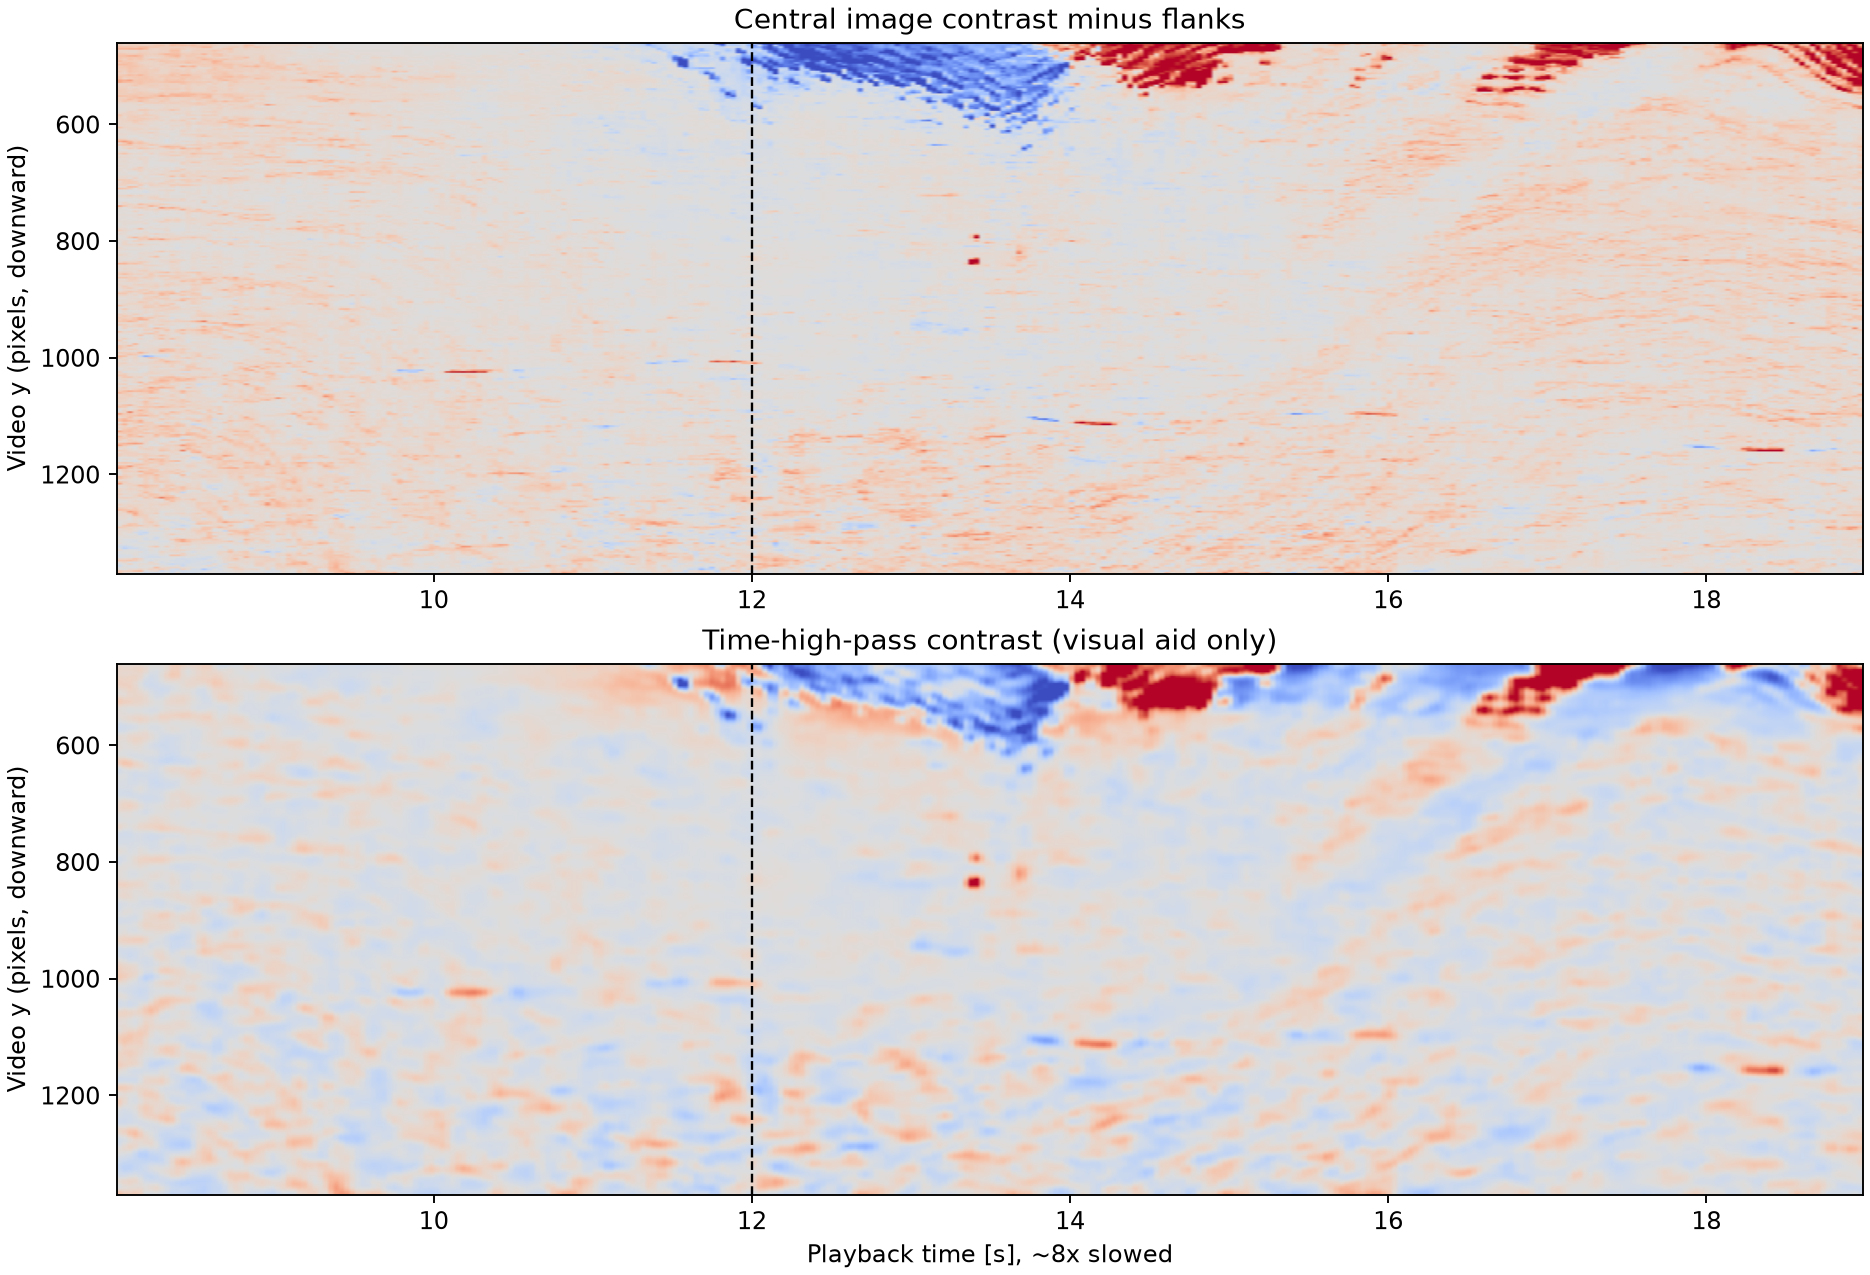
\includegraphics[width=.98\linewidth]{results/axial_kymograph.png}
\caption{Vaste ROI-analyse in video-pixels; stippellijn is 12 s \emph{afspeeltijd}. Rode/blauwe contrastbanen kunnen beweging, beeldbreking, veranderende bellenconcentratie en veranderend oppervlak voorstellen.}
\end{figure}
De contrastbanden zijn vooral in het bovenste deel uitgesproken, maar leveren geen uniek herkenbare, van onder naar boven doorlopende ridge. Optische stroom verschilt bovendien aanzienlijk tussen as en aangrenzende beeldstroken. Daarom: $v_{\mathrm{front}}=\status$. Een schatting $v=\Delta z/\Delta t$ uit de globale fotohoogte van de cilinder zou een \emph{ongegronde} golfsnelheid opleveren: $h$ is onbekend en de gebogen cilinderwand vervormt het beeld.

\section{Analytische controledynamica}
Als de vloeistof volledig met de cilinder zou meedraaien ($u_\phi=\Omega_0r$), volgt voor de vrije oppervlakte:
\begin{equation}
\eta(R)-\eta(0)=\frac{\Omega_0^2R^2}{2g},\quad R=0.075\,\mathrm m.
\end{equation}
Bij $33\,\mathrm{rpm}$ volgt $\Delta\eta=3.425\,\mathrm{mm}$ en $\Omega_0=3.456\,\mathrm{rad\,s^{-1}}$. Een langere lichtverstrooiende trechter is dus \emph{niet} zonder verdere analyse het oppervlak van deze uniforme achtergrond. Lokale kerndynamica en/of bellenstructuren zijn belangrijk.

De standaard referentie voor lineaire vrije inertiële golven in een uniform roterende bulk is
\begin{align}
\omega_{\mathrm I}&=\pm2\Omega_0\frac{k_z}{\sqrt{k_r^2+k_z^2}},\qquad
\big|\omega_{\mathrm I}\big|\leq2\Omega_0,\\
\big|v_{g,z}\big|&=\left|\frac{\partial\omega_{\mathrm I}}{\partial k_z}\right|
=\frac{2\Omega_0 k_r^2}{(k_r^2+k_z^2)^{3/2}}.
\end{align}
Een radiaal gestructureerde axiale golf kan dus axiale groepsvoortplanting vertonen, ook zonder een schuin reizende centrale as. De frequentieband bij 33 rpm is $|\omega|\leq6.91\,\mathrm{rad\,s^{-1}}$ of $|f|\leq1.10\,\mathrm{Hz}$ in het meedraaiende stelsel. Dit is een \emph{controlemodel}; de werkelijke waterproef bevat viscositeit, grenzen en een vrij oppervlak \cite{Greenspan1968,Yang2020}.

Voor water met $\nu\simeq10^{-6}\,\mathrm{m^2\,s^{-1}}$ is een eenvoudige diffusielengte na $1.5\,\mathrm s$ ongeveer $\sqrt{\nu t}=1.22\,\mathrm{mm}$. Snelle centimeterveranderingen zijn daarmee niet door \emph{puur lokaal diffunderen} verklaard; massa-transport en vloeistofdynamische koppeling blijven toegelaten alternatieven.

\section{Preregistratie volgende falsifier}
\textbf{Doel:} is er een pulsspecifiek coherent axiaal fasefront met een voortplantingssnelheid die onafhankelijk van bellenadvectie en uniforme rotatie wordt gemeten? De nulhypothese is dat het zichtbare patroon door advectie, spin-up en oppervlakte/bellenrespons kan worden verklaard.
\begin{enumerate}[leftmargin=*,nosep]
\item Behoud A070 v0.2.2 en zijn bestaande SHA-256-locks \emph{ongewijzigd}. De huidige, reeds bekeken video blijft alleen exploratieve data.
\item Leg minimaal vier condities geblindeerd vast: constante rotatie, sham-puls, positieve rotorpuls, negatieve rotorpuls; richtgetal acht herhalingen per conditie.
\item Registreer onafhankelijke rotortachometer of encoder, rotorcommandotijdstip, waterdiepte, rotorstraal, watertemperatuur, beltoevoer en synchrone zij- en bovencamera.
\item Meet minimaal drie hoogtes langs de as met onafhankelijke fase- of tracermetingen; meet waterspiegelhoogte afzonderlijk van de bellenkolom.
\item Vergelijk preregistreerd: $t_{\rm arr}\propto z$ (propagatie), $t_{\rm arr}\propto z^2$ (diffusief referentiemodel), en tracergemeten advectie; kwalificeer radiale inertiële modi en de frequentieband $|\omega|\leq2\Omega_0$.
\item Verzegel classificatie en fits voordat trial labels en rotorlogs worden onthuld; publiceer raw data, code, hashes, niet-geslaagde controles en onzekerheden.
\end{enumerate}
\noindent\textbf{Beslisregel:} geen kandidaat-torsiepuls zonder repliceerbare, onafhankelijke fasevertraging over meerdere hoogtes en zonder scheiding van bellen-/traceradvectie. Ook een bevestigde watergolf bewijst geen lichttorsie; die SST-claim vereist een afzonderlijke \emph{inviscide} finite-core-PKLSA-oplossing, zonder $c$, $r_c$ of de canonieke swirlsnelheid als tuninginput.
\section{Gatekaart}
\small
\begin{tabularx}{\linewidth}{@{}p{1.0cm}X@{}}
\toprule
Gate & Afsluitvoorwaarde \\\midrule
G0--G2 & dataprovenance, frame-/plaatskalibratie en onafhankelijke pulsaanvang \\
G3--G4 & tracer/bellen-scheiding en controle tegen sham/steady-run \\
G5--G7 & fasevertraging, axiale groepsvoortplanting en vergelijking met advectie, diffusie en inertiële modi \\
G8--G9 & vrije-oppervlakhoogte afzonderlijk en $m$-mode uit bovencamera \\
G10 & nieuwe bron-native inviscide finite-core torsieproef, slechts na bovenstaande kwalificatie \\
G11 & koppeling aan Swirl Clock, operationele afstand en licht blijft \textbf{UNRESOLVED} \\
\bottomrule
\end{tabularx}
\normalsize
\paragraph{Status.} Vijf technische regressiechecks van de \emph{observatie-extractor} slagen. De fysieke gates G0--G11 zijn niet uitgevoerd. Het video-materiaal is niet blind ten opzichte van de waarnemer. De v0.2.3-map is een preregistratieplan, \emph{geen} gegenereerde framework-v1.0.7-productie-instance.
\begin{thebibliography}{9}\small
\bibitem{Yang2020} W. Yang, I. Delbende, Y. Fraigneau, and L. Martin Witkowski (2020),
``Large axisymmetric surface deformation and dewetting in the flow above a rotating disk in a cylindrical tank: Spin-up and permanent regimes,''
\emph{Physical Review Fluids} \textbf{5}, 044801.
\href{https://doi.org/10.1103/PhysRevFluids.5.044801}{doi:10.1103/PhysRevFluids.5.044801}.
\bibitem{Greenspan1968} H. P. Greenspan (1968), \emph{The Theory of Rotating Fluids}, Cambridge University Press. ISBN 9780521043885.
\bibitem{Batchelor1967} G. K. Batchelor (1967), \emph{An Introduction to Fluid Dynamics}, Cambridge University Press. \href{https://doi.org/10.1017/CBO9780511800955}{doi:10.1017/CBO9780511800955}.
\end{thebibliography}
\end{document}
